%
\documentclass[11pt]{article}

% The usual packages
\usepackage{booktabs}
\usepackage{array}
\usepackage{subcaption}

\usepackage{fullpage}
\usepackage{breakcites}
\usepackage{setspace}
\usepackage{endnotes}
\usepackage{mathtools} % for \mathclap
%\usepackage{float} % can't use with floatrow
\usepackage{amsmath}
\usepackage{amsfonts}
\usepackage{amssymb}
\usepackage{rotating}
\usepackage{longtable}
\usepackage{microtype}
\usepackage{graphicx}
\usepackage{hyperref}
%\usepackage[usenames,dvipsnames]{color}
\usepackage{url}
\usepackage{natbib}
\usepackage{framed}
\usepackage{epigraph}
\usepackage{lipsum}
\usepackage{textcomp} % for \textrightarrow
\usepackage{dcolumn}
\usepackage{nameref}
\usepackage{booktabs}
\usepackage{float}
%\restylefloat{table}
\bibpunct{(}{)}{;}{a}{}{,}

% kable packages
\usepackage{booktabs}
\usepackage{longtable}
\usepackage{array}
\usepackage{multirow}
\usepackage[table]{xcolor}
\usepackage{wrapfig}
\usepackage{float}
\usepackage{colortbl}
\usepackage{pdflscape}
\usepackage{tabu}
\usepackage{threeparttable}
\usepackage{threeparttablex}
\usepackage[normalem]{ulem}
\usepackage{makecell}

% Set paragraph spacing the way I like
\parskip=0pt
\parindent=20pt

%\usepackage{helvet}
%\usepackage[labelfont={bf}, margin=0cm, font=small, skip=0pt]{caption}

\newcommand\numberthis{\addtocounter{equation}{1}\tag{\theequation}}

% Define mathematical results
\newtheorem{lemma}{Lemma}
\newtheorem{proposition}{Proposition}
\newtheorem{theorem}{Theorem}
\newtheorem{claim}{Claim}
\newenvironment{proof}[1][Proof]{\begin{trivlist}
\item[\hskip \labelsep {\bfseries #1}]}{\end{trivlist}}
\newenvironment{definition}[1][Definition]{\begin{trivlist}
\item[\hskip \labelsep {\bfseries #1}]}{\end{trivlist}}
\newenvironment{example}[1][Example]{\begin{trivlist}
\item[\hskip \labelsep {\bfseries #1}]}{\end{trivlist}}
\newenvironment{remark}[1][Remark]{\begin{trivlist}
\item[\hskip \labelsep {\bfseries #1}]}{\end{trivlist}}
\DeclareMathOperator*{\argmin}{arg\,min}
\DeclareMathOperator{\med}{med}
\DeclareMathOperator*{\E}{\text{E}}
%\DeclareMathOperator*{\Pr}{\text{Pr}}

%Set up fonts the way I like
%\usepackage{tgpagella}
%\usepackage[T1]{fontenc}
%\usepackage[bitstream-charter]{mathdesign}

%% Baskervald
%\usepackage[lf]{Baskervaldx} % lining figures
%\usepackage[bigdelims,vvarbb]{newtxmath} % math italic letters from Nimbus Roman
%\usepackage[cal=boondoxo]{mathalfa} % mathcal from STIX, unslanted a bit
%\renewcommand*\oldstylenums[1]{\textosf{#1}}

%\usepackage[T1]{fontenc}
%\usepackage{newtxtext,newtxmath}

% A special command to create line break in table cells
\newcommand{\specialcell}[2][c]{%
 \begin{tabular}[#1]{@{}c@{}}#2\end{tabular}}

%% Set up lists the way I like
% Redefine the first level
\renewcommand{\theenumi}{\arabic{enumi}.}
\renewcommand{\labelenumi}{\theenumi}
% Redefine the second level
\renewcommand{\theenumii}{\alph{enumii}.}
\renewcommand{\labelenumii}{\theenumii}
% Redefine the third level
\renewcommand{\theenumiii}{\roman{enumiii}.}
\renewcommand{\labelenumiii}{\theenumiii}
% Redefine the fourth level
\renewcommand{\theenumiv}{\Alph{enumiv}.}
\renewcommand{\labelenumiv}{\theenumiv}
% Eliminate spacing around lists
\usepackage{enumitem}
\setlist{nolistsep}

% Create footnote command so that my name
% has an asterisk rather than a one.
\long\def\symbolfootnote[#1]#2{\begingroup%
\def\thefootnote{\fnsymbol{footnote}}\footnote[#1]{#2}\endgroup}
%\usepackage{footmisc}
%\renewcommand{\thefootnote}{\symbolfootnote{footnote}}

% Create the colors I want
\usepackage{color, xcolor}
\definecolor{color1}{RGB}{217,95,2}  % orange
\definecolor{color2}{RGB}{27,158,119}  % green
\definecolor{color3}{RGB}{117,112,179}  % purple

% for colored \left( and \right)
\newcommand{\cleft}[2][.]{%
  \begingroup\colorlet{savedleftcolor}{.}%
  \color{#1}\left#2\color{savedleftcolor}%
}
\newcommand{\cright}[2][.]{%
  \color{#1}\right#2\endgroup
}

% for drawing arrows
\usepackage{tikz}
\usetikzlibrary{calc,shapes}

\newcommand{\tikzmark}[1]{\tikz[overlay,remember picture] \node (#1) {};}
\newcommand{\DrawBox}[2]{%
  \begin{tikzpicture}[overlay,remember picture]
    \draw[->,shorten >= 6pt, shorten <= 2pt, out=-90, in=85, distance=1.3cm, color2, thick] (MarkA.east) to (MarkB.east);
    \draw[->,shorten >= 6pt, shorten <= 2pt, out=-90, in=90, distance=1cm, color2, thick] (MarkC.west) to (MarkD.east);
  \end{tikzpicture}
}

% remarks by equations
\newcommand{\justif}[2]{&{#1}&\text{#2}}


% set up pdf
\hypersetup{
pdftitle={}, % title
pdfauthor={Carlisle Rainey}, % author
pdfkeywords={bias} {first difference} {marginal effect} {quantities of interest} {maximum likelihood}
pdfnewwindow=true, % links in new window
colorlinks=true, % false: boxed links; true: colored links
linkcolor=black, % color of internal links
citecolor=black, % color of links to bibliography
filecolor=blue, % color of file links
urlcolor=blue % color of external links
}

% section headers
%\usepackage[scaled]{helvet}
%\renewcommand\familydefault{\sfdefault}
%\usepackage[T1]{fontenc}
%\usepackage{titlesec}
%\titleformat{\section}
%  {\normalfont\sffamily\Large\bfseries}
%  {\thesection}{1em}{}
%\titleformat{\subsection}
%  {\normalfont\sffamily\large\bfseries}
%  {\thesection}{1em}{}
%  \titleformat{\subsubsection}
%  {\normalfont\sffamily\bfseries}
%  {\thesection}{1em}{}

% enable comments in pdf
\newcommand{\dtk}[1]{\textcolor{blue}{#1}}
\newcommand{\ctk}[1]{\textcolor{red}{#1}}

\begin{document}

\begin{center}

{\Large \textbf{Simulation-Induced Bias in Quantities of Interest}}\symbolfootnote[1]{All computer code necessary for replication is available on \href{https://github.com/carlislerainey/unnecessary}{GitHub}. We thank Bill Berry, Christopher Gandrud, Michael Hanmer, John Holbein, Gary King, Justin Kirkland, Thomas Leeper, Matt Pietryka, Arthur Spirling, Michael Tomz, Jason Wittenberg, and Chris Wlezien for helpful comments. We also thank audiences at Florida State University and the 2018 Texas Methods Meeting for productive discussions. All remaining errors are our own.}

\vspace{1cm}

Carlisle Rainey\symbolfootnote[2]{Carlisle Rainey is Associate Professor of Political Science, Florida State University, 540 Bellamy, Tallahassee, FL, 32306. (\href{mailto:crainey@fsu.edu}{crainey@fsu.edu}).}

\vspace{2mm}

Holger L. Kern\symbolfootnote[3]{Holger L. Kern is Assistant Professor of Political Science, Florida State University, 541 Bellamy, Tallahassee, FL, 32306. (\href{mailto:hkern@fsu.edu}{hkern@fsu.edu}).}

\vspace{1cm}

\today
\end{center}

\vspace{5mm}

% Abstract
{\centerline{\textbf{Abstract}}}
\begin{quote}\noindent
Following \cite{KingTomzWittenberg2000} researchers commonly obtain point estimates of quantities of interest by simulating model coefficients, transforming these simulated coefficients into simulated quantities of interest, and then taking the average of the simulated quantities of interest. In contrast, other researchers directly transform coefficient estimates into estimated quantities of interest using the invariance property of maximum likelihood estimators. These approaches are not equivalent. We show both analytically and empirically that computing quantities of interest using the average of simulations can introduce substantial bias. To avoid this bias, researchers can use the invariance property to calculate maximum likelihood estimates of quantities of interest.\\
\end{quote}

% Add quote to first page
% \epigraph{}

%\begin{center}
%Manuscript word count:
%\end{center}

% Remove page number from first page
\thispagestyle{empty}

% Start main text
%\newpage
%\doublespace
\onehalfspace
%\section*{Introduction}

Political scientists employ maximum likelihood (ML) to estimate a variety of statistical models. ML estimators have desirable and widely understood properties. Researchers fit several common models with ML, including logit and probit models (along with their ordered and multinomial variants), Poisson and negative binomial models, and many varieties of duration models. Even least-squares corresponds to the ML estimates for the normal-linear model. Political scientists (e.g., \citealt{KatzKing1999}, \citealt{Mebane2000}, and \citealt{Sartori2003})  commonly  rely ML estimators to fit theoretically motivated statistical models. But for many research questions, the model coefficient estimates are not the quantities of greatest interest to the researcher.

\cite{KingTomzWittenberg2000} urges researchers to focus on substantively meaningful quantities of interest, such as predicted probabilities, expected counts, marginal effects, and first differences, and provides a method to compute these quantities and the associated uncertainty. Before the publication of \cite{KingTomzWittenberg2000} and the development of CLARIFY for Stata \citep{TomzWittenbergKing2003} and Zelig for R (\citealt{ImaiKingLau2008}; \citealt{Choiratetal}), political scientists tended to report lengthy tables of coefficient estimates and pay little attention to the substantive meaning of the estimates beyond their sign and statistical significance.

This foundational work spawned a swath of extensions of the method and software implementations. For example, \cite{Licht2011} extends King, Tomz, and Wittenberg's simulation-based approach to Cox proportional hazard models, and \cite{Gandrud2015} develops the software to implement the method. \cite{WilliamsWhitten2012} describes how researchers can use simulation to more fully understand dynamic models of time-series cross-sectional data, and \cite{WilliamsWhitten2011} implements their suggestions. 

\cite{KingTomzWittenberg2000} had a tremendous impact on substantive research as well. Citations demonstrate its broad usage. As of September 2018, Google Scholar lists 3,746 citations for \cite{KingTomzWittenberg2000} 1,487 citations for \cite{TomzWittenbergKing2003}, making it one of the most cited political methodology articles. Further Google Scholar lists 1,487 citations for \cite{TomzWittenbergKing2003}, 349 citations for \cite{ImaiKingLau2008}, and 334 citations for \cite{Choiratetal}. In short, the valuable advice offered by \cite{KingTomzWittenberg2000} has influenced many scholars and improved research in political science and the social sciences more generally.

In addition to focusing researchers on more relevant quantities of interest, \cite{KingTomzWittenberg2000} popularized the simulation-based approach to compute these quantities of interest. With the simulation-based approach, researchers simulate model coefficients, transform these simulated coefficients into simulated quantities of interest, and finally summarize the distribution of the simulated quantities of interest.

Our paper addresses one aspect of the advice in \cite{KingTomzWittenberg2000}: to use the average of the simulated quantities of interest as the point estimator. We refer to this estimator as the ``average of simulations.'' We show both analytically and empirically that averaging simulations compounds the transformation-induced bias that \cite{Rainey2017} describes. Researchers can easily avoid compounding the transformation-induced bias by using ML estimates of quantities of interest rather than the average of simulations. Researchers can easily obtain estimates of the quantities of interest from coefficient estimates using the invariance property of ML estimators.

The invariance property of ML estimators allows a researcher to find the ML estimate of a function of a parameter by first using ML to estimate the model parameter and then applying the function to that estimate (\citealt[pp.\@ 75--76]{King1989}; \citealt[pp.\@ 320--321]{CasellaBerger2002}). More formally, suppose a researcher uses ML to estimate a statistical model in which $y_i \sim f(\theta_i)$, where $i \in \{1,\ldots, N\}$ and $f$ represents a probability distribution. The parameter $\theta_i$ connects to a design matrix $X$ of $k$ explanatory variables and a column of ones by a link function $g(\cdot)$, so that $g(\theta_i) = X_i\beta$, where $\beta \in \mathbb{R}^{k+1}$ represents a vector of parameter with length $k + 1$. The researcher uses ML to compute estimates $\hat{\beta}^{\text{mle}}$ for the parameter vector $\beta$. We denote the function that transforms model coefficients into quantities of interest as $\tau(\cdot)$. For example, if the researcher uses a logit model and focuses on the predicted probability for a specific observation $X_c$, then $\tau(\beta) = \text{logit}^{-1}( X_c \beta) = \dfrac{1}{1 + e^{-X_c\beta}}$. The researcher can use the invariance property to quickly obtain a ML estimate of the predicted probability: $\hat{\tau}^{\text{mle}} = \tau \left( \hat{\beta}^{\text{mle}}\right) = \text{logit}^{-1} \left( X_c \hat{\beta}^{\text{mle}} \right) = \dfrac{1}{1 + e^{-X_c \hat{\beta}^{\text{mle}}}}$.

Software implementations differ in whether they rely on the invariance property or \cite{KingTomzWittenberg2000}'s simulation-based approach. Several software packages, such as the \texttt{margins} command in Stata \citep{StataManual}, the margins package in R \citep{margins}, and the \texttt{predict()} function in R for the glm \citep{R} and polr \citep{MASS} classes, uses the invariance property. Other software packages, such as CLARIFY for Stata \citep{TomzWittenbergKing2003} and Zelig for R (\citealt{ImaiKingLau2008}; \citealt{Choiratetal}), report the average of simulations. In the Stata code to create marginal effects plots for a probit model, \cite{BramborClarkGolder2006} use the average of simulations.

The methodological literature is similarly divided. \cite{Herron1999} uses the invariance property to derive an ML estimator for predicted probabilities in limited dependent variable models (and uses simulation to compute confidence intervals). Even though \cite{Herron1999} cites an earlier version of \cite{KingTomzWittenberg2000}, it does not mention the fact that its approach differs from \cite{KingTomzWittenberg2000}. \cite{CarseyHarden2013} follows \cite{KingTomzWittenberg2000} and uses the average of simulations. The literature seems to incorrectly treat both estimators as essentially equivalent. However, as we show, the two are not equivalent. Indeed, the ML estimator has a distinct advantage over the average of simulations.

\section*{Transformation-Induced $\tau$-Bias}

As \citet{Rainey2017} shows, using the invariance property to transform unbiased model coefficient estimates can introduce bias into estimated quantities of interest. \citet[p.\@ 404]{Rainey2017} decomposes the bias in the estimate of the quantity of interest, which he refers to as {total $\tau$-bias,} into two components: transformation-induced $\tau$-bias and coefficient-induced $\tau$-bias. \citet{Rainey2017} defines these as
\begin{equation}
\text{total } \tau\text{-bias}= \underbrace{ \E\left[\tau\left(\hat{\beta}^\text{mle}\right)\right]-  \tau\left[\E\left(\hat{\beta}^\text{mle}\right)\right]  }_{\text{transformation-induced}} + \overbrace{  \tau\left[\E\left(\hat{\beta}^\text{mle}\right)\right] - \tau\left(\beta\right)  }^{\text{coefficient-induced}}\text{.} \label{eqn:ti-bias}
\end{equation}

Transformation-induced $\tau$-bias behaves systematically. The shape of the transformation $\tau(\cdot)$ determines the direction of the bias. In general, any strictly convex (concave) $\tau(\cdot)$ creates upward (downward) transformation-induced $\tau$-bias.

The direction and magnitude of the coefficient-induced $\tau$-bias depend on the choice of $\tau(\cdot)$ and the bias in the coefficient estimates, but an unbiased estimator $\hat{\beta}^\text{mle}$ implies the absence of coefficient-induced $\tau$-bias. We consider coefficient-induced $\tau$-bias only briefly in the section ``\nameref{ci-bias}'', but set it aside for the bulk of our analysis. Instead, we extend the concept of transformation-induced bias from ML estimates to the average of simulations. 

\subsection*{The Average of Simulations}

Rather than rely on the invariance property of ML estimators to compute a point estimate for a quantity of interest, \cite{KingTomzWittenberg2000} suggests the following simulation-based approach:\vspace{.1in}
\begin{enumerate}
\item \textit{Fit the model.}
Use ML to estimate the model coefficients $\hat{\beta}^{\text{mle}}$ and their covariance $\hat{V} \left( \hat{\beta}^{\text{mle}} \right)$.
\item \textit{Simulate the coefficients.}
Simulate a large number $M$ of coefficient vectors $\tilde{\beta}^{(i)}$, for $i \in \{1, 2,\ldots, M\}$, using $\tilde{\beta}^{(i)} \sim \text{MVN} \left[ \hat{\beta}^{\text{mle}}, \hat{V} \left( \hat{\beta}^{\text{mle}} \right) \right]$, where MVN represents the multivariate normal distribution.
\item \textit{Convert simulated coefficients into simulated quantity of interest.}
Compute $\tilde{\tau}^{(i)} = \tau \left( \tilde{\beta}^{(i)} \right)$ for $i \in \{1, 2,\ldots, M\}$.
Most quantities of interest depend on the values of the explanatory variables. In this situation, researchers either focus on a specific observation (typically some kind of ``average case'') or average across all sample observations \citep{HanmerKalkan2013}. In any case, the transformation $\tau(\cdot)$ includes this choice.\footnote{As \cite{KingTomzWittenberg2000} note, this step might require additional simulation, to first introduce and then average over fundamental uncertainty. We ignore this additional step since it does not affect our argument.} \item \textit{Average the simulations of the quantity of interest.} Estimate the quantity of interest using the average of the simulations of the quantity of interest, so that $\hat{\tau}^{\text{avg}} = \frac{1}{M} \sum_{i = 1}^{M} \tilde{\tau}^{(i)}$.\footnote{In the discussion that follows, we assume no Monte Carlo error exists in $\hat{\tau}^{\text{avg}}$. In other words, we assume that $M$ is sufficiently large so that $\hat{\tau}^{\text{avg}} = \text{E}\left[ \tau \left(\tilde{\beta} \right) \right]$, where $\tilde{\beta} \sim \text{MVN} \left[ \hat{\beta}^{\text{mle}}, \hat{V} \left( \hat{\beta}^{\text{mle}} \right) \right]$.}\\
\end{enumerate}

\section*{A Definition of Simulation-Induced Bias}

The literature offers two ways to estimate quantities of interest: (1) calculate the ML estimator $\hat{\tau}^\text{mle}$ using the invariance property of ML estimators or (2) calculate the average of simulations $\hat{\tau}^\text{avg}$ using the algorithm described in \cite{KingTomzWittenberg2000}. How does $\hat{\tau}^\text{avg}$ compare to $\hat{\tau}^{\text{mle}}$?

If the transformation of coefficient estimates into an estimate of the quantity of interest is always convex (or always concave), then Jensen's inequality allows the simple statement relating $\hat{\tau}^\text{avg}$ and $\hat{\tau}^{\text{mle}}$ given in Lemma \ref{lem:direction} .

\begin{lemma}\label{lem:direction}
Suppose a nondegenerate ML estimator $\hat{\beta}^\text{mle}$.
Then any strictly convex (concave) $\tau(\cdot)$ guarantees that $\hat{\tau}^{\text{avg}}$ is strictly greater (less) than $\hat{\tau}^\text{mle}$.
\end{lemma}
\begin{proof}
By definition, $$ \hat{\tau}^{\text{avg}} = \text{E}\left[ \tau \left(\tilde{\beta} \right) \right].$$
Using Jensen's inequality \citep[p.\@ 190, Thm.\@ 4.7.7]{CasellaBerger2002}, we know that $\text{E}\left[ \tau \left(\tilde{\beta} \right) \right] > \tau \left[ \text{E}\left( \tilde{\beta} \right) \right]$, so that $$\hat{\tau}^{\text{avg}} > \tau \left[ \text{E}\left( \tilde{\beta} \right) \right].$$
However, because $\tilde{\beta} \sim \text{MVN} \left[ \hat{\beta}^{\text{mle}}, \hat{V} \left( \hat{\beta}^{\text{mle}} \right) \right]$, $\text{E}\left( \tilde{\beta} \right) = \hat{\beta}^\text{mle}$, so that
$$\hat{\tau}^{\text{avg}} > \tau \left( \hat{\beta}^\text{mle}\right).$$
Of course, $\hat{\tau}^\text{mle} = \tau \left( {\hat{\beta}^\text{mle}} \right)$ by definition, so that $$\hat{\tau}^{\text{avg}} > \hat{\tau}^\text{mle}.$$
The proof for concave $\tau$ follows similarly.
 $\blacksquare$
\end{proof}

\noindent This result is intuitive. Since we simulate using a multivariate normal distribution, $\tilde{\beta}$ has a symmetric distribution. By definition, $\hat{\tau}^\text{mle}$ equals the mode of the distribution of $\tau(\tilde{\beta})$. But the distribution of $\tau(\tilde{\beta})$ is \emph{not} symmetric. If $\tilde{\beta}$ happens to fall below the mode $\hat{\beta}^\text{mle}$, then $\tau(\cdot)$ pulls $\tau(\tilde{\beta})$ in toward $\hat{\tau}^\text{mle}$.
If $\tilde{\beta}$ happens to fall above the mode $\hat{\beta}^\text{mle}$, then $\tau(\cdot)$ pushes $\tau(\tilde{\beta})$ away from $\hat{\tau}^\text{mle}$. This creates a right-skewed distribution for $\tau(\tilde{\beta})$, which pushes the average $\hat{\tau}^\text{avg}$ above $\hat{\tau}^\text{mle}$.

For a convex transformation, Lemma \ref{lem:direction} shows that $\hat{\tau}^\text{avg}$ is always larger than $\hat{\tau}^\text{mle}$. We refer to the expectation of this difference between $\hat{\tau}^\text{avg}$ and $\hat{\tau}^\text{mle}$ as ``simulation-induced bias," so that
\begin{align*}
\text{simulation-induced } \tau\text{-bias} =& \E \left(\hat{\tau}^\text{avg} \right) - \E \left(\hat{\tau}^\text{mle} \right).
\end{align*}

Theorem \ref{thm:direction} compares the sum of simulation- and transformation-induced $\tau$-bias in $\hat{\tau}^\text{avg}$ to transformation-induced $\tau$-bias in $\hat{\tau}^\text{avg}$.

\begin{theorem}\label{thm:direction}
Suppose a nondegenerate ML estimator $\hat{\beta}^\text{mle}$.
Then for any strictly convex or concave $\tau(\cdot)$, the sum of the simulation-induced and transformation-induced $\tau$-bias in $\hat{\tau}^{\text{avg}}$ is strictly greater in magnitude than the transformation-induced $\tau$-bias in $\hat{\tau}^{\text{mle}}$.
\end{theorem}
\begin{proof}
According to Theorem 1 of \citet[p.\@ 405]{Rainey2017}, $\E \left( \hat{\tau}^\text{mle}\right) -  \tau \left[\E \left( \hat{\beta}^\text{mle} \right) \right] > 0$.
Lemma \ref{lem:direction} shows that for any convex $\tau$, $\hat{\tau}^{\text{avg}} > \hat{\tau}^\text{mle}$.
It follows that $\underbrace{\E \left( \hat{\tau}^\text{avg}\right) - \tau \left[\E \left( \hat{\beta}^\text{mle} \right) \right]}_{\text{s.i. and t.i. } \tau\text{-bias in }\hat{\tau}^{\text{avg}}} > \underbrace{\E \left( \hat{\tau}^\text{mle}\right) -  \tau \left[\E \left( \hat{\beta}^\text{mle} \right) \right]}_{\text{t.i. } \tau\text{-bias in }\hat{\tau}^{\text{mle}}} > 0$.\\

\noindent For the concave case, it follows similarly that $\underbrace{\E \left( \hat{\tau}^\text{avg}\right) - \tau \left[\E \left( \hat{\beta}^\text{mle} \right) \right]}_{\text{s.i. and t.i. } \tau\text{-bias in }\hat{\tau}^{\text{avg}}} < \underbrace{\E \left( \hat{\tau}^\text{mle}\right) -  \tau \left[\E \left( \hat{\beta}^\text{mle} \right) \right]}_{\text{t.i. } \tau\text{-bias in }\hat{\tau}^{\text{mle}}} < 0$.
 $\blacksquare$
\end{proof}
Regardless of the direction the simulation-induced and transformation-induced $\tau$-bias, Theorem \ref{thm:direction} shows that the magnitude of the combination in $\hat{\tau}^{\text{avg}}$
is \textit{always} larger than the transformation-induced bias alone in  $\hat{\tau}^{\text{mle}}$ for strictly convex or concave $\tau(\cdot)$. 

\section*{An Approximation of Simulation-Induced Bias}

Theorem \ref{thm:direction} shows that $\hat{\tau}^\text{avg}$ compounds both transformation-induced $\tau$-bias with simulation-induced $\tau$-bias. But is this bias substantively important? Monte Carlo experiments allow us to assess this directly, but an analytical approximation provides a helpful guideline.
We approximate the simulation-induced $\tau$-bias in $\hat{\tau}^\text{avg}$ as
\begin{align*}
\text{simulation-induced $\tau$-bias in } \hat{\tau}^\text{avg} =& \underbrace{\left( \E \left( \hat{\tau}^\text{avg}\right) - \tau \left[\E \left( \hat{\beta}^\text{mle} \right) \right] \right) }_{\text{t.i. } \tau\text{-bias in }\hat{\tau}^{\text{avg}}} - \underbrace{ \left( \E \left( \hat{\tau}^\text{mle}\right) -  \tau \left[\E \left( \hat{\beta}^\text{mle} \right) \right] \right)}_{\text{t.i. } \tau\text{-bias in }\hat{\tau}^{\text{mle}}}\\
=& \E \left( \hat{\tau}^\text{avg}\right) - \E \left( \hat{\tau}^\text{mle}\right)\\
=& \E \left( \hat{\tau}^\text{avg} - \hat{\tau}^\text{mle} \right)\\
=& \E \left(     \E \left[ \tau\left( \tilde{\beta} \right) \right]      -      \tau \left( \hat{\beta}^\text{mle} \right)     \right)\\
=& \E \left(     \underbrace{\E \left[ \tau\left( \tilde{\beta} \right) \right]      -      \tau \left[ E\left(  \tilde{\beta} \right)\right]}_{\substack{\text{approximated in Eq. 1,} \\ \text{p. 405, of \cite{Rainey2017}}}}   \right)\\
\approx & \E \left[ \dfrac{1}{2} \displaystyle \sum_{r = 1}^{k+1} \sum_{s = 1}^{k+1} H_{rs}\left( \hat{\beta}^\text{mle} \right) \hat{V}_{rs} \left( \hat{\beta}^{\text{mle}} \right) \right], \numberthis \label{eqn:avg-approx}
\end{align*}
where the remaining expectation occurs with respect to $\hat{\beta}^\text{mle}$, $H\left( \hat{\beta}^\text{mle} \right)$ represents the Hessian matrix of second derivatives of $\tau(\cdot)$ at the point $\hat{\beta}^\text{mle}$ and, conveniently, $\hat{V} \left( \hat{\beta}^{\text{mle}} \right)$ represents the estimated covariance matrix for $\hat{\beta}^\text{mle}$.

This approximation appears similar to the approximation for the transformation-induced $\tau$-bias, which (adjusting notation slightly) \citet[p. 405, Eq. 1]{Rainey2017} computes as
\begin{align*}
\text{t.i. } \tau \text{-bias } \approx \dfrac{1}{2} \displaystyle \sum_{r = 1}^{k+1} \sum_{s = 1}^{k+1} H_{rs}\left[ \E \left( \hat{\beta}^\text{mle} \right) \right] V_{rs} \left( \hat{\beta}^{\text{mle}} \right), \numberthis \label{eqn:mle-approx}
\end{align*}
where $H\left[ \E \left( \hat{\beta}^\text{mle} \right) \right]$ represents the Hessian matrix of second derivatives of $\tau(\cdot)$ at the point $\E \left( \hat{\beta}^\text{mle} \right)$ and $V \left( \hat{\beta}^{\text{mle}} \right)$ represents the covariance matrix of the sampling distribution of $\hat{\beta}^\text{mle}$.

When we compare Equations \ref{eqn:avg-approx} and \ref{eqn:mle-approx}, we yet again compare the \textit{expectation of a function} with the \textit{function of the expectation}.
Therefore, Equations \ref{eqn:avg-approx} and \ref{eqn:mle-approx} are not exactly equal.
But, as a rough guideline, we should expect them to be similar.
And to the extent that the two are similar, the additional simulation-induced $\tau$-bias in $\hat{\tau}^\text{avg}$ is about the same as the transformation-induced $\tau$-bias in $\hat{\tau}^\text{mle}$. 

Because of the similarity between Equations \ref{eqn:avg-approx} and \ref{eqn:mle-approx}, the simulation-induced $\tau$-bias becomes large under the conditions identified by \cite{Rainey2017} as leading to large transformation-induced $\tau$-bias: when the non-linearity in the transformation $\tau(\cdot)$ is severe and when the standard errors of $\hat{\beta}^\text{mle}$ are large.
While the transformation-induced $\tau$-bias vanishes as the number of observations grows large, it can be substantively meaningful for the sample sizes commonly encountered in social science research \citep{Rainey2017}.

\section*{The Intuition of Simulation-Induced Bias}

\subsection*{Using a Drastic, Convex Transformation: $\tau(\mu) = \mu^2$}

To develop an intuition for the simulation-induced $\tau$-bias in $\hat{\tau}^\text{avg}$, consider the simple scenario in which $y_i \sim \text{N}(0, 1)$, for $i \in \{1, 2, \ldots, n = 100\}$, and the researcher wishes to estimate $\mu^2$. Suppose that the researcher knows that the variance equals one but does not know that the mean $\mu$ equals zero. The researcher uses the unbiased maximum likelihood estimator $\hat{\mu}^\text{mle} = \frac{\sum_{i=1}^n y_i}{n}$ of $\mu$, but ultimately cares about the quantity of interest $\tau(\mu) = \mu^2$. The researcher can use the invariance property to compute the ML estimate $\tau(\mu)$ as $\hat{\tau}^\text{mle} = \left( \hat{\mu}^\text{mle} \right) ^2$. Alternatively, the researcher can use the simulation-based approach, estimating $\tau(\mu)$ as $\hat{\tau}^\text{avg} = \frac{1}{M} \sum_{i = 1}^M \tau \left( \tilde{\mu}^{(i)} \right)$, where $\tilde{\mu}^{(i)} \sim \text{N} \left( \hat{\mu}^\text{mle}, \frac{1}{\sqrt{n}} \right)$ for $i \in \{1, 2,\ldots, M\}$.

The true value of the quantity of interest is $\tau(0) = 0^2 = 0$. However, the ML estimator $\hat{\tau}^\text{mle} = \left( \hat{\mu}^\text{mle} \right)^2$ equals zero if and only if $\hat{\mu}^\text{mle} = 0$. Otherwise, $\hat{\tau}^\text{mle} > 0$. Since $\hat{\mu}^\text{mle}$ almost surely differs from zero,  $\hat{\tau}^\text{mle}$ is biased upward.

Moreover, even if $\hat{\mu}^\text{mle} = 0$, $\tilde{\mu}^{(i)}$ almost surely differs from zero. If $\tilde{\mu}^{(i)} \neq 0$, then $\left( \tilde{\mu}^{(i)} \right)^2 > 0$. Thus, $\hat{\mu}^\text{avg}$ is almost surely larger than the true value $\tau(\mu) = 0$ even when $\hat{\mu} = 0$.

We illustrate this fact clearly by repeatedly simulating $y$ and computing $\hat{\tau}^\text{mle}$ and $\hat{\tau}^\text{avg}$. Figure \ref{fig:int} shows the first four of 10,000 total simulations. The figure shows how the unbiased estimate $\hat{\mu}^\text{mle}$ is translated into $\hat{\tau}^\text{mle}$ and $\hat{\tau}^\text{avg}$.

First, to find $\hat{\tau}^\text{avg}$, we complete three steps: (1) simulate $\tilde{\mu}^{(i)} \sim \text{N} \left( \hat{\mu}^\text{mle}, \frac{1}{10{}} \right)$ for $i \in \{1, 2,\ldots, M = 1,000\}$, (2) calculate $\tilde{\tau}^{(i)} = \tau\left( \tilde{\mu}^{(i)} \right)$, and (3) calculate $\hat{\tau}^\text{avg} = \frac{1}{M} \sum_{i = 1}^M \tilde{\tau}^{(i)}$. The rug plot along the horizontal axis shows the distribution of $\tilde{\mu}$. The hollow points in Figure \ref{fig:int} shows the transformation of each point $\tilde{\mu}^{(i)}$ into $\tilde{\tau}^{(i)}$. The rug plot along the vertical axis shows the distribution of $\tilde{\tau}$.
Focus on the top-left panel of Figure \ref{fig:int}. Notice that $\hat{\mu}^\text{mle}$ estimates the true value $\mu = 0$ quite well. However, after simulating $\tilde{\mu}$ and transforming $\tilde{\mu}$ into $\tilde{\tau}$, the $\tilde{\tau}$s fall far from the true value $\tau(0) = 0$. The dashed orange line shows the average of $\tilde{\tau}$. Notice that although $\hat{\mu}^\text{mle}$ is unusually close to the truth $\mu = 0$ in this sample, $\hat{\tau}^\text{avg}$ is substantially biased upward.

\begin{figure}[h]
\begin{center}
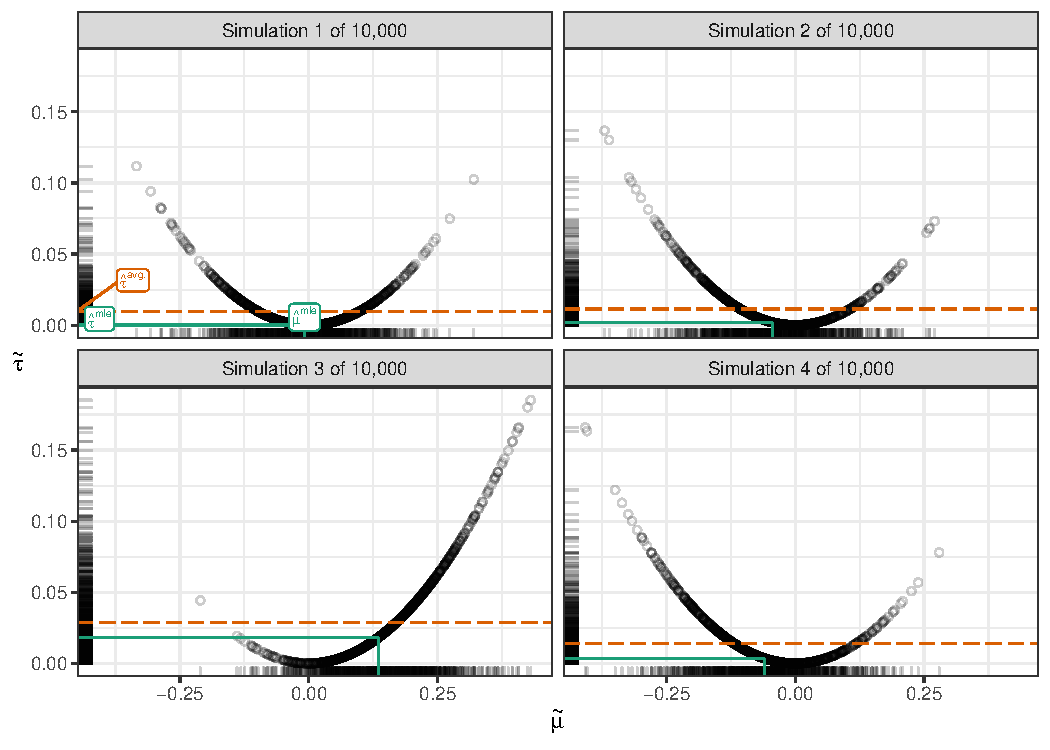
\includegraphics[width = \textwidth]{figs/intuition.pdf}\\
\vspace{.1in}
\caption{The first four Monte Carlo simulations of $\hat{mu}$. These four panels illustrate the relationship between $\hat{\tau}^\text{mle}$ and $\hat{\tau}^\text{avg}$ described by Lemma \ref{lem:direction} and Theorem \ref{thm:direction}.}\label{fig:samp}
\end{center}
\end{figure}

Second, to find $\hat{\tau}^\text{mle}$, we simply transform $\hat{\mu}^\text{mle}$ directly using $\hat{\tau}^\text{mle} = \left( \hat{\mu}^\text{mle} \right) ^2$.
The solid green lines show this transformation.
The convex transformation $\tau(\cdot)$ has the effect of lengthening the right tail of the distribution of $\tilde{\tau}$, pulling the average well above the mode.
This provides the basic intuition for Lemma \ref{lem:direction}.

The remaining panels of Figure \ref{fig:samp} repeat this process with three more random samples.
Each sample presents a similar story \textemdash{} the convex transformation stretches the distribution of $\tilde{\tau}$ to the right, which pulls $\hat{\tau}^\text{avg}$ above $\hat{\tau}^\text{mle}$.

We repeat this process 10,000 total times to produce 10,000 estimates $\hat{\mu}^\text{mle}$, $\hat{\tau}^\text{mle}$, and $\hat{\tau}^\text{avg}$.
Figure \ref{fig:int-samp} shows the density plots for the 10,000 estimates (i.e., the sampling distributions of $\hat{\mu}^\text{mle}$, $\hat{\tau}^\text{mle}$, and $\hat{\tau}^\text{avg}$).
As we know analytically, $\hat{\mu}^\text{mle}$ is unbiased with a standard error of $\frac{\sigma}{\sqrt{n}} = \frac{1}{\sqrt{100}} = \frac{1}{10}$.
Both $\hat{\tau}^\text{mle}$ and $\hat{\tau}^\text{avg}$ are biased upward, but $\hat{\tau}^\text{avg}$ is about twice as biased.
Theorem \ref{thm:direction} shows why this must be the case.

\begin{figure}[h]
\begin{center}
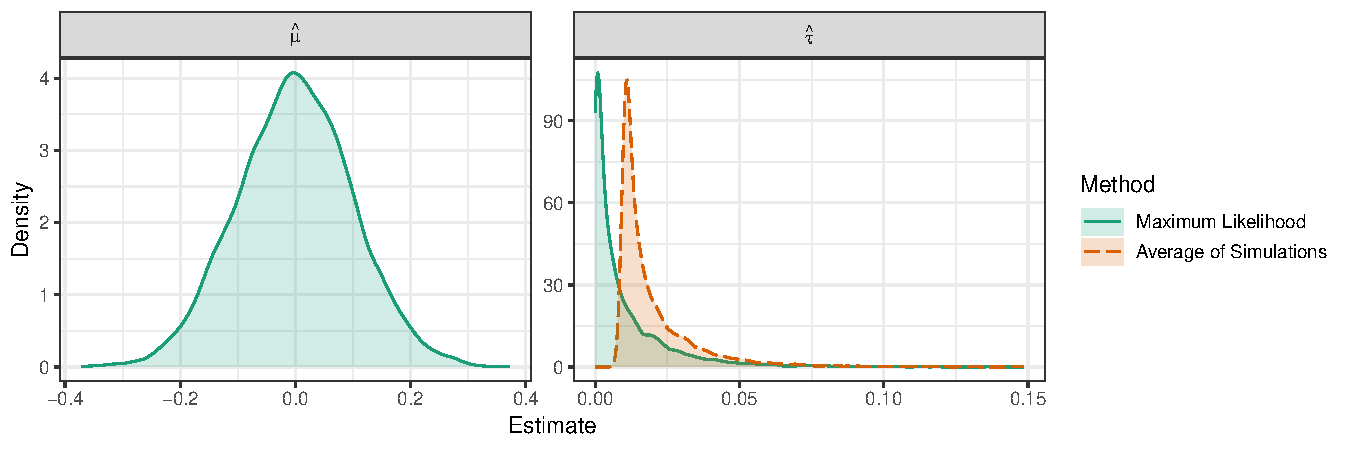
\includegraphics[width=\textwidth]{figs/intuition-sampling.pdf}\\
\vspace{.1in}
\caption{The sampling distributions of $\hat{\beta}^\text{mle}$, $\hat{\tau}^\text{mle}$, and $\hat{\tau}^\text{avg}$.}\label{fig:int-samp}
\end{center}
\end{figure}

\subsection*{Using the Law of Iterated Expectations}

Alternatively, we can develop the intuition behind our argument analytically via the law of iterated expectations. It helps to alter the notation slightly, making two implicit dependencies explicit. We explain each change below and use the alternate, more expansive notation only in this section.

The law of iterated expectations states that $\E_Y \left( \E_{X \mid Y}(X \mid Y) \right) = \E_X(X)$, where $X$ and $Y$ represent random variables.
The three expectations occur with respect to three different distributions: $\E_Y$ denotes the expectation with respect to the marginal distribution of $Y$, $\E_{X \mid Y}$ denotes the expectation with respect to the conditional distribution of $X \mid Y$, and $\E_X$ denotes the expectation with respect to the marginal distribution of $X$.

Outside of this section, we understand that the distribution of $\tilde{\beta}$ depends on $\hat{\beta}^\text{mle}$ and could be written as $\tilde{\beta} \mid \hat{\beta}^\text{mle}$.
To remain consistent with previous work, especially \cite{KingTomzWittenberg2000} and \cite{Herron1999}, we use $\tilde{\beta}$ to represent $\tilde{\beta} \mid \hat{\beta}^\text{mle}$.
The definition of $\tilde{\beta}$ makes this usage clear.
In this section only, we use $\tilde{\beta} \mid \hat{\beta}^\text{mle}$ to represent the conditional distribution of $\tilde{\beta}$ and use $\tilde{\beta}$ to represent the \underline{un}conditional distribution of $\tilde{\beta}$.
Intuitively, one might imagine (1) generating a data set $y$, (2) estimating $\hat{\beta}^\text{mle}$, and (3) simulating $\tilde{\beta} \mid \hat{\beta}^\text{mle}$.
If we do steps (1) and (2) just once, but step (3) repeatedly, we have a sample from the conditional distribution $\tilde{\beta} \mid \hat{\beta}^\text{mle}$.
If we do steps (1), (2), and (3) repeatedly, then we have a sample from the \underline{un}conditional distribution $\tilde{\beta}$.
The unconditional distribution helps us understand the nature of the simulation-induced $\tau$-bias.

Applying the law of iterated expectations, we obtain $\E_{\tilde{\beta}} \left( \tilde{\beta} \right) = \E_{\hat{\beta}^\text{mle}}\left( \E_{\tilde{\beta} \mid \hat{\beta}^\text{mle}} (\tilde{\beta} \mid \hat{\beta}^\text{mle}) \right)$.
The three identities below connect the three key quantities from Theorem \ref{thm:direction} to three versions of $\E_{\hat{\beta}^\text{mle}}\left( \E_{\tilde{\beta} \mid \hat{\beta}^\text{mle}} (\tilde{\beta} \mid \hat{\beta}^\text{mle}) \right)$, with the transformation $\tau(\cdot)$ applied at different points.
\small
\begin{alignat}{2}
 \color{color1} \tikzmark{MarkA}\tau \left[ \normalcolor \E_{\hat{\beta}^\text{mle}}\left( \E_{\tilde{\beta} \mid \hat{\beta}^\text{mle}} \left( \tilde{\beta} \mid \hat{\beta}^\text{mle} \right) \right) \color{color1} \right] \normalcolor =&  \tau \left[ \E_{\tilde{\beta}} \left( \tilde{\beta} \right) \right] = \tau \left[\E \left( \hat{\beta}^\text{mle} \right) \right]\text{,} \label{eqn:true}\\
 \E_{\hat{\beta}^\text{mle}}\left( \color{color1} \tikzmark{MarkB}\tau\tikzmark{MarkC} \left[ \normalcolor \E_{\tilde{\beta} \mid \hat{\beta}^\text{mle}} \left( \tilde{\beta} \mid \hat{\beta}^\text{mle} \right) \color{color1} \right] \normalcolor \right)  =&  \E_{\hat{\beta}^\text{mle}} \left( \tau \left[\hat{\beta}^\text{mle} \right] \right) =  \E_{\hat{\beta}^\text{mle}} \left(\hat{\tau}^\text{mle} \right) \text{, and} \justif{\quad}{$\longleftarrow~$ Switch $\tau$ and an $\E$ once.} \label{eqn:mle}\\
\E_{\hat{\beta}^\text{mle}}\left( \E_{\tilde{\beta} \mid \hat{\beta}^\text{mle}} \left( \color{color1} \tikzmark{MarkD}\tau \left[ \normalcolor \tilde{\beta} \mid \hat{\beta}^\text{mle} \color{color1} \right] \normalcolor \right) \right)  =&
\E_{\tilde{\beta}} \left( \tau \left[\tilde{\beta} \right] \right)  =
\E_{\tilde{\beta}} \left(\hat{\tau}^\text{avg} \right) \text{.}\justif{\quad}{$\longleftarrow~$ Switch $\tau$ and an $\E$ again.}\label{eqn:avg}\DrawBox{red}{blue}
\end{alignat}
\normalsize

If we subtract Equation \ref{eqn:mle} from Equation \ref{eqn:true}, we obtain the transformation-induced $\tau$-bias in $\hat{\tau}^\text{mle}$ (see Equation \ref{eqn:ti-bias} for the definition of transformation-induced $\tau$-bias).
To move from Equation \ref{eqn:true} to Equation \ref{eqn:mle} we must swap $\tau(\cdot)$ with an expectation once.
This implies that, if $\tau(\cdot)$ is convex, Equation \ref{eqn:mle} must be greater than Equation \ref{eqn:true}.
This, in turn, implies that the bias is positive.

To obtain the $\tau$-bias in $\hat{\tau}^\text{avg}$ we must subtract Equation \ref{eqn:avg} from Equation \ref{eqn:true}.
But to move from Equation \ref{eqn:true} to Equation \ref{eqn:avg} we must swap $\tau(\cdot)$ with an expectation \emph{twice}.
Again, if $\tau(\cdot)$ is convex, then Equation \ref{eqn:avg} must be greater than Equation \ref{eqn:true}.
However, because we expect $\hat{\beta}^\text{mle}$ and $\tilde{\beta} \mid \hat{\beta}^\text{mle}$ to have similar distributions, we should expect the additional swap to roughly double the bias in $\hat{\tau}^\text{avg}$ compared to $\hat{\tau}^\text{mle}$. It is this additional swap that leads to simulation-induced $\tau$-bias.

\section*{Illustrations of Simulation-Induced Bias}

To establish that simulation-induced $\tau$-bias is more than a theoretical curiosity, we use three illustrations to show that simulation-induced $\tau$-bias can matter substantively. First, we reproduce a published analysis from \cite{Holland2015} to show that the average of simulations can meaningfully differ from the ML estimate. Second, we perform a Monte Carlo analysis estimates of marginal effects from a simple Poisson regression to show that the magnitude of the bias can exceed the truth. Third, we compute the coefficient-, transformation-, and simulation-induced bias for estimates of first-differences from a realistic logistic regression to show that simulation-induced bias (1) behaves similarly to transformation-induced bias and (2) can remain even for samples large enough to essentially eliminate coefficient-induced bias.

\subsection*{Reanalysis of Holland (2015)}

Holland (2015) presents a nuanced theory that describes the conditions under which politicians choose to enforce laws and supports the theoretical argument with a rich variety of evidence. In particular, it elaborates on the \textit{electoral} incentives of politicians to enforce laws. We borrow three Poisson regressions and hypotheses about a single explanatory variable to illustrate how the ML estimate can differ from the simulation average.

Holland writes: 
\begin{quote}
My first hypothesis is that enforcement operations drop off with the fraction of poor residents in an electoral district. So district poverty should be a negative and significant predictor of enforcement, but only in politically decentralized cities [Lima and Santiago]. Poverty should have no relationship with enforcement in politically centralized cities [Bogota] once one controls for the number of vendors.
\end{quote}

To evaluate this claim, we refit Model 1 from Table 2 in \cite{Holland2015} for each city. We use each model to compute the percent increase in the enforcement operations for each district in the city if the percent of the district in the lower class dropped by half. For example, in the Villa Maria El Triunfo district in Lima, 84\% of the district is in the lower class. If this dropped to 42\%, then the average of simulations suggests that the number of enforcement operations would increase by about 284\% (from about 5 to about 19). The ML estimate, on the other hand, suggests an increase of 264\% (from about 5 to about 17). The ML estimate, then, is about 7\% smaller than the simulation average---a noticeable shrinkage. 

\begin{figure}[h]
\begin{center}
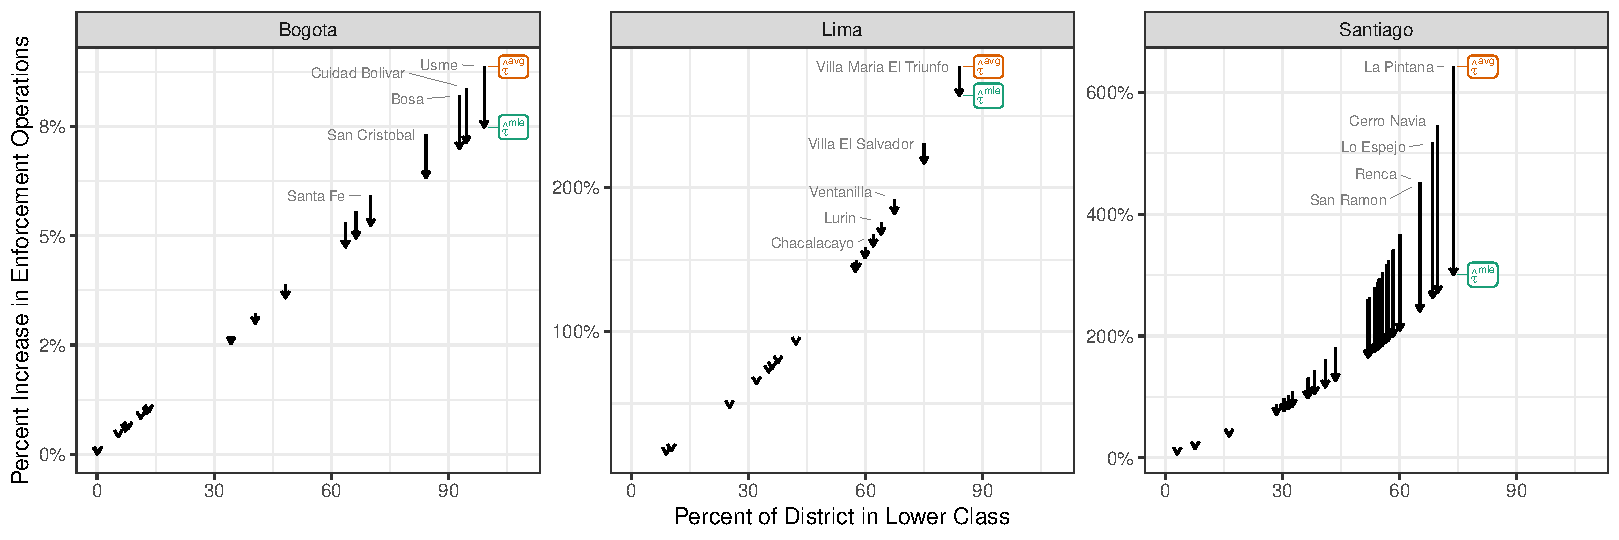
\includegraphics[width=\textwidth]{figs/holland.pdf}\\
\vspace{.1in}
\caption{This figure compares the average of simulations with the ML estimate using three Poisson regression models from Holland (2015). The quantity of interest is the percent increase in the enforcement operations when the percent of a district in the lower class drops by half. The arrows show how the estimates change when we switch from the average of simulations to the ML estimate.}\label{fig:holland}
\end{center}
\end{figure}

Figure \ref{fig:holland} shows how the estimates change (usually shrink) for all districts when we switch from the averages of simulations to ML estimates. Table \ref{tab:top-5} presents the details for the labelled cases in Figure \ref{fig:holland}. In Bogota, the estimate shrinks by 9\% in Sante Fe and 14\% in Usme. In Lima, the estimate shrinks by 4\% in Chacalacayo and 7\% Villa Maria El Triunfo. The shrinkage is much larger in Santiago, where the standard errors for the coefficient estimates are much larger. The estimate shrinks by about 47\% in San Ramon and 53\% in La Pintana. The median shrinkage is 7\% in Bogota, 2\% in Lima, and 36\% in Santiago. For many districts in Santiago, the average of simulations is about \textit{twice} the ML estimate. These estimates clearly show that the average of simulations and the ML estimates can meaningfully differ in actual analyses.

\begin{table}[!h]

\caption{\label{tab:}\label{tab:top-5}This table presents the details for the districts labelled in Figure \ref{fig:holland}.}
\centering
\fontsize{8}{10}\selectfont
\begin{tabular}[t]{>{\bfseries}l>{\bfseries}lccccccc}
\toprule
\multicolumn{2}{c}{\bfseries  } & \multicolumn{3}{c}{\bfseries Average of Simulations} & \multicolumn{3}{c}{\bfseries ML Estimate} & \multicolumn{1}{c}{\bfseries  } \\
\cmidrule(l{2pt}r{2pt}){3-5} \cmidrule(l{2pt}r{2pt}){6-8}
\textbf{City} & \textbf{District} & \textbf{\% Change\textsuperscript{a}} & \textbf{From\textsuperscript{b}} & \textbf{To\textsuperscript{c}} & \textbf{\% Change} & \textbf{From} & \textbf{To} & \textbf{Shrinkage\textsuperscript{d}}\\
\midrule
 & Usme & 9\% & 5.5 & 5.8 & 7\% & 5.4 & 5.8 & 14\%\\

 & Cuidad Bolivar & 8\% & 6.1 & 6.4 & 7\% & 5.9 & 6.3 & 13\%\\

 & Bosa & 8\% & 7.1 & 7.4 & 7\% & 6.9 & 7.4 & 13\%\\

 & San Cristobal & 7\% & 12.7 & 13.4 & 6\% & 12.5 & 13.3 & 11\%\\

\multirow{-5}{*}{\raggedright\arraybackslash Bogota} & Santa Fe & 6\% & 27.3 & 28.9 & 5\% & 26.6 & 28.0 & 9\%\\
\cmidrule{1-9}
 & Villa Maria El Triunfo & 284\% & 5.2 & 19.4 & 264\% & 4.7 & 17.1 & 7\%\\

 & Villa El Salvador & 230\% & 7.2 & 23.3 & 217\% & 6.8 & 21.4 & 6\%\\

 & Ventanilla & 192\% & 8.4 & 23.4 & 182\% & 8.2 & 23.0 & 5\%\\

 & Lurin & 176\% & 6.9 & 17.4 & 168\% & 6.4 & 17.1 & 5\%\\

\multirow{-5}{*}{\raggedright\arraybackslash Lima} & Chacalacayo & 167\% & 6.7 & 16.4 & 159\% & 6.2 & 16.1 & 4\%\\
\cmidrule{1-9}
 & La Pintana & 642\% & 1.4 & 4.0 & 301\% & 0.8 & 3.4 & 53\%\\

 & Cerro Navia & 546\% & 1.5 & 4.3 & 272\% & 1.0 & 3.6 & 50\%\\

 & Lo Espejo & 517\% & 1.4 & 4.4 & 263\% & 1.0 & 3.5 & 49\%\\

 & Renca & 452\% & 1.3 & 4.1 & 241\% & 1.0 & 3.4 & 47\%\\

\multirow{-5}{*}{\raggedright\arraybackslash Santiago} & San Ramon & 452\% & 1.2 & 4.0 & 241\% & 1.0 & 3.3 & 47\%\\
\bottomrule
\multicolumn{9}{l}{\textsuperscript{a} Quantity of interest; percent change in enforcement operations when the percent in the lower class drops by half.}\\
\multicolumn{9}{l}{\textsuperscript{b} Enforcement operations when the percent in the lower class equals its observed value.}\\
\multicolumn{9}{l}{\textsuperscript{c} Enforcement operations when the percent in the lower class equals half its observed value.}\\
\multicolumn{9}{l}{\textsuperscript{d} Shrinkage in the quantity of interest due to switching from the average of simulations to the ML estimator.}\\
\end{tabular}
\end{table}

\subsection*{Stylized Example from Rainey (2017)}

To illustrate transformation-induced bias, Rainey (2017) considers the simple, fictional model
\begin{equation}
\log (\text{income}_i) = \beta_{cons} + \beta_{edu} \text{education}_i + \epsilon_i \text{,}\nonumber
\end{equation}
where $\epsilon_i \sim N(0, \sigma^2)$, education is measured in years, and income is measured in thousands of dollars. 
Rainey uses the invariance property to compute ML estimates of the median income among those with 20 years of education $\med(\text{income} ~|~ \text{education} = 20) = e^{\beta_{cons} + 20\beta_{edu}}$. 
Following Rainey, we suppose that $N = 10$, $\beta_{cons} = 2.5$, $\beta_{edu} = 0.1$, $\sigma^2 = 1$, and education takes on integers roughly uniform from 10 to 20.
In this case, $\tau(\beta_{cons}, \beta_{edu}) = e^{\beta_{cons} + 20\beta_{edu}} \approx \$90k$. 

We use Monte Carlo simulation to obtain the sampling distributions of $\hat{\tau}^\text{mle}$ and $\hat{\tau}^\text{avg}$. As in Rainey (2017), we find that $\hat{\tau}^\text{mle}$ is biased upward by about \$15k. But we find that that average of simulations is biased upward by about \$33k. We know from statistical theory that there is no coefficient-induced $\tau$-bias in this example. Because this transformation is strictly convex, we know from Rainey (2017) that the transformation-induced $\tau$-bias is positive. Similarly, our Lemma \ref{lem:direction} reveals that every average of simulations must be greater than the associated ML estimate. Therefore, our Theorem \ref{thm:direction} reveals that the \textit{expectation} of the average of simulation must be greater than the expectation of the (upwardly biased) ML estimator. Further, notice that, consistent with our approximation, the bias in the average of simulation is about twice the bias in the ML estimator.

\begin{figure}[h!]
\begin{center}
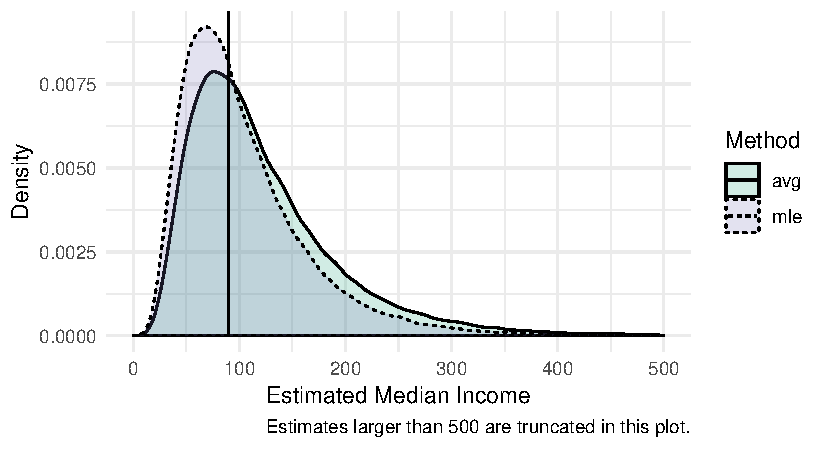
\includegraphics[scale = 0.75]{figs/rainey-2017-density.pdf}\\
\vspace{.1in}
\caption{This figure shows the sampling distributions of the average of simulations and the ML estimator of $\med(\text{income} \mid \text{education} = 20)$. The labels indicate the true value $\tau$ of about \$90k (in black) and the expectations of the the ML estimate $\hat{\tau}^\text{mle}$ of about \$105k (in green) and the average of simulations $\hat{\tau}^\text{avg}$ of about \$122k (in orange).}\label{fig:rainey-2017-density}
\end{center}
\end{figure}

\subsection*{First Differences in a Logistic Regression Model}

Next, we illustrate our concepts for a more complex, realistic logistic regression model. 
To obtain a plausible data-generating process and realistic set of explanatory variables, we base our Monte Carlo study on estimates and data from \cite{BerryDeMerittEsarey2010}. 
This paper serves as an ideal example because it is widely cited, uses a large data set, and builds on a familiar series of substantive and methodological papers, including \cite{WolfingerRosenstone1980}, \cite{Nagler1991, Nagler1994}, and \cite{AltmanMcDonald2003}.
For our data-generating process, we use the model specification and coefficients that \cite{BerryDeMerittEsarey2010} reports in their Table 1, Column 2. 
To generate suitably-small samples of explanatory variables, we randomly draw a sample of $100$ observations and subsequently add in $100$ more , then $200$ more, and then $400$ more observations to create samples of $100$, $200$, $400$, and $800$ observations from the original data set from \cite{BerryDeMerittEsarey2010}.

In our Monte Carlo simulations, we keep the explanatory variables fixed and use the coefficient estimates from \cite{BerryDeMerittEsarey2010} to simulate 10,000 outcome variables. For each simulated outcome variable, we compute $\hat{\beta}$, $\hat{\tau}^\text{mle}$, and $\hat{\tau}^\text{avg}$. Finally, we use these estimates to decompose the $\tau$-bias into its coefficient-induced, transformation-induced, and simulation-induced components.

As our quantity of interest, we calculate the change in the probability of turning out to vote if the election registration deadline occurs $10$ days sooner (a one standard deviation change). 
However, the effect of this 10-day shift (and the coefficient-, transformation-, and simulation-induced $\tau$-bias) depends on the original closing date as well as the values of the other explanatory variables. To capture and present this heterogeneity, we estimate the coefficient-, transformation-, and simulation-induced biases for 250 randomly-chosen observations from the full data set. 

Figure \ref{fig:nagler} shows the resulting coefficient-, transformation-, and simulation-induced $\tau$-bias (columns) for the four different sample sizes (rows). Each point shows the bias for one of the 250 observations. Points that fall outside the shaded region have a bias greater than $10\%$. 

\begin{figure}[h!]
\begin{center}
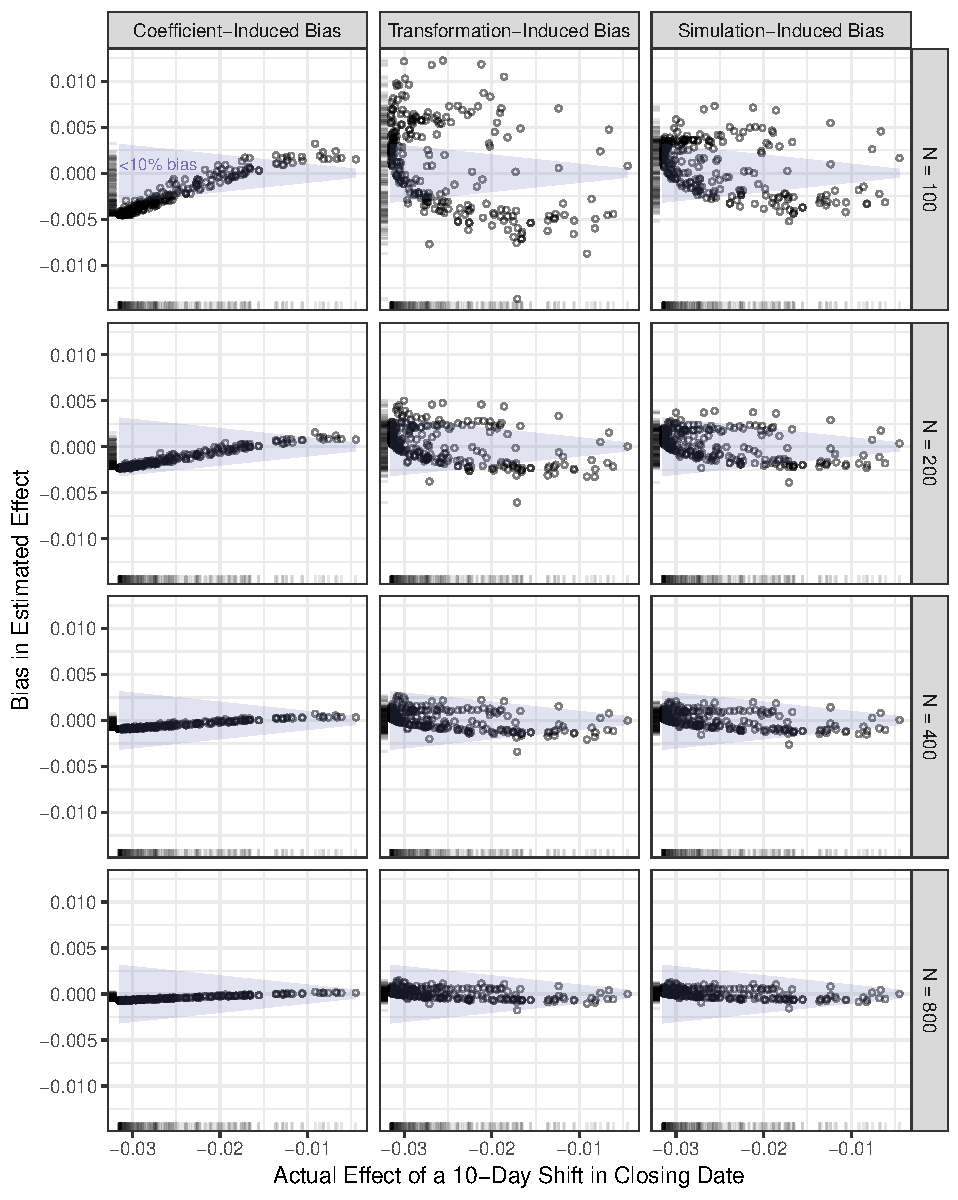
\includegraphics[scale = 0.75]{figs/nagler-fd-bias.pdf}\\
\vspace{.1in}
\caption{The figure shows the coefficient-induced, transformation-induced, and simulation-induced $\tau$-biases for a logistic regression model based on \cite{BerryDeMerittEsarey2010}.
The points that fall outside the shaded region have bias greater than $10\%$.}\label{fig:nagler}
\end{center}
\end{figure}

First, note that the simulation-induced $\tau$-bias (right-hand column) has a magnitude comparable to the well-known small sample bias in logistic regression coefficients (left-hand column). The magnitude of the simulation-induced $\tau$-bias is similar to the magnitude of the transformation-induced $\tau$-bias (middle column), in line with our approximation. Second, at least in some scenarios, the simulation-induced bias is sufficiently large to meaningfully affect results. For at least some observations, the simulation-induced bias remains larger than $10\%$ until the sample size exceeds $400$. Third, while each type of bias disappears asymptotically, the biases disappear at different rates. Rainey (2017) shows that transformation-induced bias can disappear more slowly than coefficient-induced bias. We see the same pattern for simulation-induced bias. Especially for certain observations, the simulation-induced bias remains large even when the coefficient-induced bias has nearly disappeared. 

\section*{A Note on \cite{HanmerKalkan2013}}

\cite{HanmerKalkan2013} recommend that researchers avoid the {\it average-case} approach for computing quantities of interest and instead use the {\it observed-value} approach. With either approach, researchers estimate the quantity of interest as a key explanatory variable changes its value. However, with non-linear models, researchers must also consider the other explanatory variables in the model since they alter the quantity of interest. The average-case approach sets the other explanatory variables to central values such as the mean, median, or mode. \cite{HanmerKalkan2013}, in contrast, suggests estimating the quantity of interest for all sample observations, leaving the explanatory variables except for the key variable of interest at their observed values, and then averaging the estimates across the sample. Here, our notation captures this choice as part of the transformation $\tau(\cdot)$, so Hanmer and Kalkan's (compelling) argument does not undermine or enhance our own.\footnote{We generally agree with the arguments in favor of the observed-value approach but recommend that researchers plot the distribution of quantities of interest in addition to providing a summary measure such as their average. See \cite{AiNorton2003} for discussion and examples.}

Because researchers have not drawn a sharp conceptual distinction between the simulation average estimator and the ML estimator, \cite{HanmerKalkan2013} does not discuss this choice. Since it explicitly builds on \cite{KingTomzWittenberg2000}, we interpret \cite{HanmerKalkan2013} as relying on the simulation average estimator when computing quantities of interest. The replication archive for the article confirms that this is indeed the case.

The important point is this: \cite{HanmerKalkan2013} draws a distinction between the average-case and observed-value approaches to computing quantities of interest. Our paper draws a distinction between computing estimates of quantities of interest (whether average-case or observed-value based) using the invariance property of ML estimators or using King, Tomz, and Wittenberg's (2000) simulation-based approach. Regardless of whether researchers use the average-case approach or the observed-value approach, the simulation-based approach leads to estimates that include simulation-induced bias that researchers can easily avoid by relying on the invariance property of ML estimators instead.

\section*{A Note of Caution}\label{ci-bias}

Our analysis focuses on the bias in estimators of quantities of interest. In particular, we focus additional bias attributable averaging simulations--what we call simulation-induced bias. We urge caution along three dimensions. 

First, we remain agnostic about the best strategy to compute standard errors and confidence intervals. Commonly employed approaches include the delta method, simulation, and the bootstrap (e.g., \cite{EfronTibshirani1993}. For example, the margins package \citep{margins} in R reports ML estimates of the quantities of interest, but allows the user to choose among the delta method (default), simulation, and the bootstrap.
\cite{KrinskyRobb1991} presents some limited Monte Carlo evidence that these approaches lead to similar inferences, but the literature has not offered a detailed comparison of these approaches.

Second, the presence of simulation-induced $\tau$-bias (and the transformation-induced $\tau$-bias of Rainey [2017]) does not always imply greater total $\tau$-bias. Indeed, the three sources of $\tau$-bias (simulation-induced, transformation-induced, and coefficient-induced) can cancel, so that just the right amount of simulation- and transformation-induced $\tau$-bias can cancel the coefficient-induced $\tau$-bias. Indeed, simulation- and transformation-induced $\tau$-bias can work much like Firth's (\citeyear{Firth1993}) modified score function to correct the coefficient-induced $\tau$-bias.

Third, applied researchers care about more than bias. In particular, they care about both bias and \textit{variance}. What can we say about the effects of simulation and transformation on the variance? In particular, what about the effect on the mean squared error (MSE)?

At first, it might seem like an estimator that is strictly greater than an upwardly biased estimator cannot have a smaller MSE. But this intuition is wrong. 

Suppose a convex transformation and define $\delta = \hat{\tau}^{\text{avg}}- \hat{\tau}^\text{mle}$. In this case, $\delta$ is deterministic for a particular sample, but a random variable across samples. However, (for a convex transformation) $\delta$ is strictly positive. By defintion $\text{MSE}\left( \hat{\tau}^\text{mle}\right) = \text{E}\left[ (\hat{\tau}^\text{mle} - \tau)^2\right]$. Similarly, $\text{MSE}\left( \hat{\tau}^\text{avg}\right) = \text{E}\left[ (\hat{\tau}^\text{avg} - \tau)^2\right]$. We can manipulate $\text{MSE}\left( \hat{\tau}^\text{avg}\right)$ as follows:
\begin{small}
\begin{align*}
\text{MSE}\left( \hat{\tau}^\text{avg}\right)&= \text{E}\left[ (\hat{\tau}^\text{mle} + \delta - \tau)^2\right] \text{ (def. of $\delta$)} \\
&= \text{E}\left[ ((\hat{\tau}^\text{mle} - \tau) + \delta)^2\right] \text{ (rearrange)} \\
&= \text{E}\left[ (\hat{\tau}^\text{mle} - \tau)^2 + 2\delta(\hat{\tau}^\text{mle} - \tau)  + \delta^2\right] \text{ (expand)} \\
&= \text{E}\left[ (\hat{\tau}^\text{mle} - \tau)^2 \right] + 2\text{E}\left[ \delta(\hat{\tau}^\text{mle} - \tau) \right]  + \text{E}\left[ \delta^2\right] \text{ (distribute expectation)} \\
&= \text{MSE}\left( \hat{\tau}^\text{mle}\right) + 2\text{E}\left[ \delta(\hat{\tau}^\text{mle} - \tau) \right]  + \text{E}\left[ \delta^2\right] \text{ (def. of MSE)} \\
\text{MSE}\left( \hat{\tau}^\text{avg}\right) - \text{MSE}\left( \hat{\tau}^\text{mle}\right)  &= 2\text{E}\left[ \delta(\hat{\tau}^\text{mle} - \tau) \right]  + \text{E}\left[ \delta^2\right] \text{ (rearrange)} \\
&= 2\text{E}\left[ \delta(\hat{\tau}^\text{mle} - \tau) \right]  + \text{E}\left[ \delta^2\right] \text{ (rearrange)} \\
&= 2 \left[ \text{E}(\delta)E(\hat{\tau}^\text{mle} - \tau) + \text{Cov}(\delta, \hat{\tau}^\text{mle} - \tau) \right]  + \text{E}\left[ \delta^2\right] \text{ (def. of covariance)} \\
&= 2 \underbrace{\text{Cov}(\delta, \hat{\tau}^\text{mle} - \tau)}_{\mathclap{\text{sign unknown}}}  + 2 \underbrace{\text{E}(\delta)}_{\mathclap{\text{positive}}} \underbrace{E(\hat{\tau}^\text{mle} - \tau)}_{\mathclap{\text{positive}}}  + \underbrace{\text{E}\left[ \delta^2\right]}_{\mathclap{\text{positive}}} \text{ (rearrange)} \numberthis\label{eqn:cov}\\
\end{align*}
\end{small}
\noindent At our level of generality, $\text{Cov}(\delta, \hat{\tau}^\text{mle} - \tau)$ can be positive or negative. If it is negative and larger than the second and third terms of Equation \ref{eqn:cov}, then the MSE for the simulation average is smaller than the ML estimator. However, this condition does not hold in general.

As an example, Figure \ref{fig:rainey-2017-summary} shows the bias, standard deviation (SD), and root mean squared error (RMSE) for the sampling distributions from Rainey (2017) shown in Figure \ref{fig:rainey-2017-density}. In this case, the average of simulations has a higher bias, SD, and RMSE. The ML estimator dominates the average of simulations. 

\begin{figure}[h!]
\begin{center}
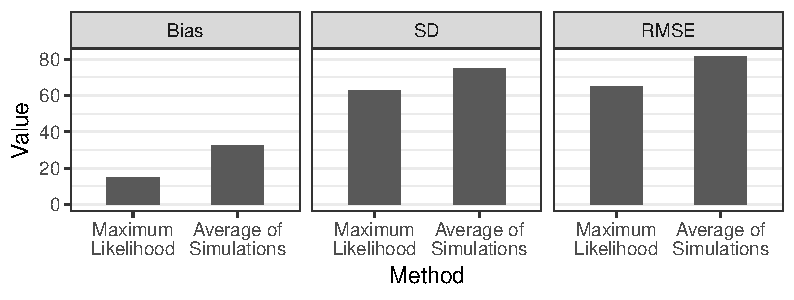
\includegraphics[scale = 0.75]{figs/rainey-2017-summary.pdf}\\
\vspace{.1in}
\caption{This figure compares the bias, SD, and RMSE of the sampling distributions of the average of simulations and the ML estimator of $\med(\text{income} \mid \text{education} = 20)$.}\label{fig:rainey-2017-summary}
\end{center}
\end{figure}

But not all cases are as simple as the stylized example from Rainey (2017). That simple scenario has an increasing, convex transformation and no coefficient-induced bias. To illustrate the complexity of the issue, we use Monte Carlo simulation to compute the bias, SD, and RMSE of estimates of marginal effects from a simple logit model. Let $\pi_i = \text{logit}^{-1}(\beta_\text{cons} + \beta_\text{x}x_i)$ for $i = \{1, 2, ..., 100\}$,  $\beta_\text{cons} = 0$, and $\beta_\text{x} = 1$. We create $x_i$ by drawing from a standard normal distribution. In this scenario, the transformation is neither increasing nor convex and the coefficients estimates have bias. Figure \ref{fig:logit-mse-me} shows the bias, variance, MSE of the estimates of the marginal effect as $x$ ranges from $-3$ to $+3$. 

\begin{figure}[h!]
\begin{center}
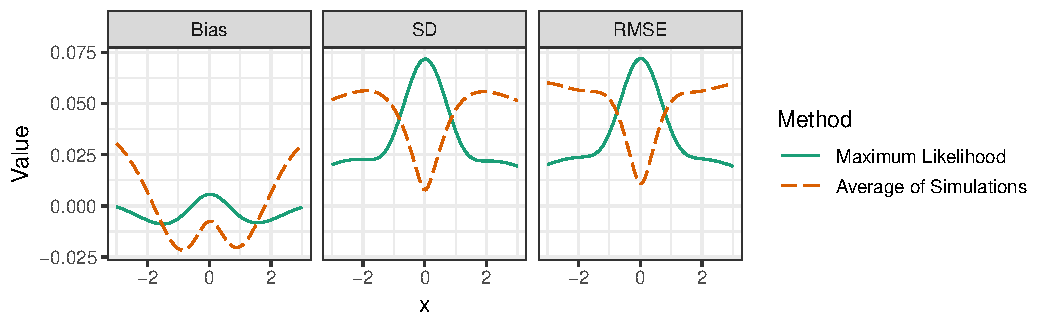
\includegraphics[scale = 0.75]{figs/logit-mse-me.pdf}\\
\vspace{.1in}
\caption{This figure compares the bias, SD, and RMSE of the sampling distributions of the simulation average and the ML estimators of the marginal effect of $x$ in a simple logit model.}\label{fig:logit-mse-me}
\end{center}
\end{figure}

\noindent In this simple simulation, the ML estimate has a smaller absolute bias for about 80\% of the range of $x$, a smaller variance in about 72\% of the range of $x$, and a smaller MSE for about 75\% of the range of $x$. Thus, in some scenarios, the average of simulations have a smaller total $\tau$-bias, RMSE, or both. Note, though, that these patterns do not necessarily generalize to other scenarios, including other statistical models, other true coefficients, and other quantities of interest. These simulations do illustrate, though, the complexity of the tradeoff.

\section*{Conclusion}

Many social scientists turn to \cite{KingTomzWittenberg2000} for advice on how to interpret, summarize, and present empirical results. By highlighting the importance of reporting substantively meaningful quantities of interest, it has significantly improved empirical research in political science and neighboring disciplines. Depending on the statistical software used, researchers estimate quantities of interest either with the average of simulated quantities of interest (e.g., Clarify in Stata, Zelig in R) or using the invariance property of ML estimators (e.g., margins in Stata and R). In practice, researchers' choice between these two estimators seems idiosyncratic rather than principled, depending on their preferred software package rather than any statistical criteria. Further, the methodological literature has not distinguished or compared the two approaches to estimating quantities of interest.

We show that when researchers use the average of simulations to estimate quantities of interest, they roughly double the transformation-induced bias that Rainey (2017) describes. We refer to this unnecessary additional bias as ``simulation-induced bias.'' The good news is that the fix is easy: we do not have to use the simulation-based approach to obtain a point estimate for a quantity of interest. Instead, we can simply plug estimated coefficients into the transformation to obtain the ML estimate of the quantity of interest. We recommend that statistical software does this by default.

\singlespace
\clearpage
\small
\bibliographystyle{apsr_fs}
\bibliography{bibliography}

\end{document}
